% ================================================================
% Chapter 1 � Model Basics
% ================================================================

\chapter{Model basics}
\label{PE}
\minitoc

\newpage
$\ $\newline    % force a new ligne

% ================================================================
% Primitive Equations
% ================================================================
\section{Primitive Equations}
\label{PE_PE}

% -------------------------------------------------------------------------------------------------------------
%        Vector Invariant Formulation 
% -------------------------------------------------------------------------------------------------------------

\subsection{Vector Invariant Formulation}
\label{PE_Vector}


The ocean is a fluid that can be described to a good approximation by the primitive 
equations, $i.e.$ the Navier-Stokes equations along with a nonlinear equation of 
state which couples the two active tracers (temperature and salinity) to the fluid 
velocity, plus the following additional assumptions made from scale considerations:

\textit{(1) spherical earth approximation: }the geopotential surfaces are assumed to 
be spheres so that gravity (local vertical) is parallel to the earth's radius

\textit{(2) thin-shell approximation: }the ocean depth is neglected compared to the earth's radius

\textit{(3) turbulent closure hypothesis: }the turbulent fluxes (which represent the effect 
of small scale processes on the large-scale) are expressed in terms of large-scale features

\textit{(4) Boussinesq hypothesis:} density variations are neglected except in their 
contribution to the buoyancy force

\textit{(5) Hydrostatic hypothesis: }the vertical momentum equation is reduced to a 
balance between the vertical pressure gradient and the buoyancy force (this removes 
convective processes from the initial Navier-Stokes equations and so convective processes 
must be parameterized instead)

\textit{(6) Incompressibility hypothesis: }the three dimensional divergence of the velocity 
vector is assumed to be zero.

Because the gravitational force is so dominant in the equations of large-scale motions, 
it is useful to choose an orthogonal set of unit vectors (\textbf{i},\textbf{j},\textbf{k}) linked 
to the earth such that \textbf{k} is the local upward vector and (\textbf{i},\textbf{j}) are two 
vectors orthogonal to \textbf{k}, $i.e.$ tangent to the geopotential surfaces. Let us define 
the following variables: \textbf{U} the vector velocity, $\textbf{U}=\textbf{U}_h + w\, \textbf{k}$ 
(the subscript $h$ denotes the local horizontal vector, $i.e.$ over the (\textbf{i},\textbf{j}) plane), 
$T$ the potential temperature, $S$ the salinity, \textit{$\rho $} the \textit{in situ} density. 
The vector invariant form of the primitive equations in the (\textbf{i},\textbf{j},\textbf{k}) 
vector system provides the following six equations (namely the momentum balance, the 
hydrostatic equilibrium, the incompressibility equation, the heat and salt conservation 
equations and an equation of state):
\begin{subequations} \label{Eq_PE}
  \begin{equation}     \label{Eq_PE_dyn}
\frac{\partial {\rm {\bf U}}_h }{\partial t}=
-\left[    {\left( {\nabla \times {\rm {\bf U}}} \right)\times {\rm {\bf U}}
            +\frac{1}{2}\nabla \left( {{\rm {\bf U}}^2} \right)}    \right]_h
 -f\;{\rm {\bf k}}\times {\rm {\bf U}}_h 
-\frac{1}{\rho _o }\nabla _h p + {\rm {\bf D}}^{\rm {\bf U}} + {\rm {\bf F}}^{\rm {\bf U}}
  \end{equation}
  \begin{equation}     \label{Eq_PE_hydrostatic}
\frac{\partial p }{\partial z} = - \rho \ g
  \end{equation}
  \begin{equation}     \label{Eq_PE_continuity}
\nabla \cdot {\bf U}=  0
  \end{equation}
\begin{equation} \label{Eq_PE_tra_T}
\frac{\partial T}{\partial t} = - \nabla \cdot  \left( T \ \rm{\bf U} \right) + D^T + F^T
  \end{equation}
  \begin{equation}     \label{Eq_PE_tra_S}
\frac{\partial S}{\partial t} = - \nabla \cdot  \left( S \ \rm{\bf U} \right) + D^S + F^S
  \end{equation}
  \begin{equation}     \label{Eq_PE_eos}
\rho = \rho \left( T,S,p \right)
  \end{equation}
\end{subequations}
where $\nabla$ is the generalised derivative vector operator in $(\bf i,\bf j, \bf k)$ directions, 
$t$ is the time, $z$ is the vertical coordinate, $\rho $ is the \textit{in situ} density given by 
the equation of state (\ref{Eq_PE_eos}), $\rho_o$ is a reference density, $p$ the pressure, 
$f=2 \bf \Omega \cdot \bf k$ is the Coriolis acceleration (where $\bf \Omega$ is the Earth's 
angular velocity vector), and $g$ is the gravitational acceleration. 
${\rm {\bf D}}^{\rm {\bf U}}$, $D^T$ and $D^S$ are the parameterisations of small-scale 
physics for momentum, temperature and salinity, and ${\rm {\bf F}}^{\rm {\bf U}}$, $F^T$ 
and $F^S$ surface forcing terms. Their nature and formulation are discussed in 
\S\ref{PE_zdf_ldf} and page \S\ref{PE_boundary_condition}.

.

% -------------------------------------------------------------------------------------------------------------
% Boundary condition
% -------------------------------------------------------------------------------------------------------------
\subsection{Boundary Conditions}
\label{PE_boundary_condition}

An ocean is bounded by complex coastlines, bottom topography at its base and an air-sea 
or ice-sea interface at its top. These boundaries can be defined by two surfaces, $z=-H(i,j)$ 
and $z=\eta(i,j,k,t)$, where $H$ is the depth of the ocean bottom and $\eta$ is the height 
of the sea surface. Both $H$ and $\eta$ are usually referenced to a given surface, $z=0$, 
chosen as a mean sea surface (Fig.~\ref{Fig_ocean_bc}). Through these two boundaries, 
the ocean can exchange fluxes of heat, fresh water, salt, and momentum with the solid earth, 
the continental margins, the sea ice and the atmosphere. However, some of these fluxes are 
so weak that even on climatic time scales of thousands of years they can be neglected. 
In the following, we briefly review the fluxes exchanged at the interfaces between the ocean 
and the other components of the earth system.

%>>>>>>>>>>>>>>>>>>>>>>>>>>>>
\begin{figure}[!ht]	 \begin{center}
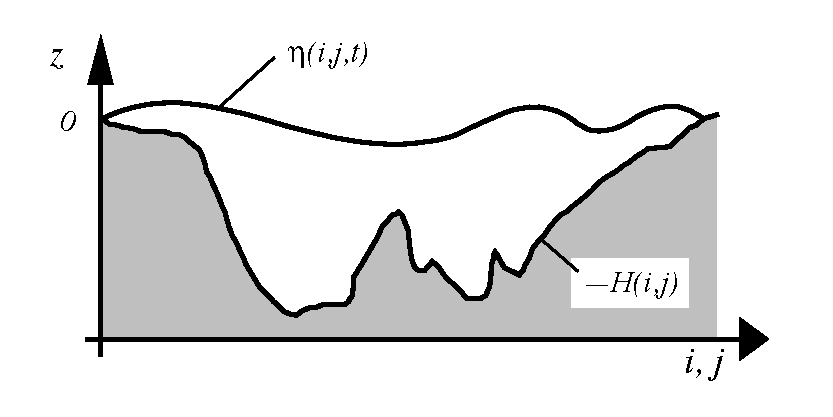
\includegraphics[width=0.90\textwidth]{./TexFiles/Figures/Fig_I_ocean_bc.pdf}
\caption{	 \label{Fig_ocean_bc} 
The ocean is bounded by two surfaces, $z=-H(i,j)$ and $z=\eta(i,j,t)$, where $H$ 
is the depth of the sea floor and $\eta$ the height of the sea surface. 
Both $H$ and $\eta$ are referenced to $z=0$.}
\end{center}   \end{figure}
%>>>>>>>>>>>>>>>>>>>>>>>>>>>>


\begin{description}
\item[Land - ocean interface:] the major flux between continental margins and the ocean is 
a mass exchange of fresh water through river runoff. Such an exchange modifies the sea 
surface salinity especially in the vicinity of major river mouths. It can be neglected for short 
range integrations but has to be taken into account for long term integrations as it influences 
the characteristics of water masses formed (especially at high latitudes). It is required in order 
to close the water cycle of the climate system. It is usually specified as a fresh water flux at 
the air-sea interface in the vicinity of river mouths.
\item[Solid earth - ocean interface:] heat and salt fluxes through the sea floor are small, 
except in special areas of little extent. They are usually neglected in the model 
\footnote{In fact, it has been shown that the heat flux associated with the solid Earth cooling 
($i.e.$the geothermal heating) is not negligible for the thermohaline circulation of the world 
ocean (see \ref{TRA_bbc}).}. 
The boundary condition is thus set to no flux of heat and salt across solid boundaries. 
For momentum, the situation is different. There is no flow across solid boundaries, 
$i.e.$ the velocity normal to the ocean bottom and coastlines is zero (in other words, 
the bottom velocity is parallel to solid boundaries). This kinematic boundary condition 
can be expressed as:
\begin{equation} \label{Eq_PE_w_bbc}
w = -{\rm {\bf U}}_h \cdot  \nabla _h \left( H \right)
\end{equation}
In addition, the ocean exchanges momentum with the earth through frictional processes. 
Such momentum transfer occurs at small scales in a boundary layer. It must be parameterized 
in terms of turbulent fluxes using bottom and/or lateral boundary conditions. Its specification 
depends on the nature of the physical parameterisation used for ${\rm {\bf D}}^{\rm {\bf U}}$ 
in \eqref{Eq_PE_dyn}. It is discussed in \S\ref{PE_zdf}, page~\pageref{PE_zdf}.% and Chap. III.6 to 9.
\item[Atmosphere - ocean interface:] the kinematic surface condition plus the mass flux 
of fresh water PE  (the precipitation minus evaporation budget) leads to: 
\begin{equation} \label{Eq_PE_w_sbc}
w = \frac{\partial \eta }{\partial t} 
    + \left. {{\rm {\bf U}}_h } \right|_{z=\eta } \cdot  \nabla _h \left( \eta \right) 
    + P-E
\end{equation}
The dynamic boundary condition, neglecting the surface tension (which removes capillary 
waves from the system) leads to the continuity of pressure across the interface $z=\eta$. 
The atmosphere and ocean also exchange horizontal momentum (wind stress), and heat.
\item[Sea ice - ocean interface:] the ocean and sea ice exchange heat, salt, fresh water 
and momentum. The sea surface temperature is constrained to be at the freezing point 
at the interface. Sea ice salinity is very low ($\sim4-6 \,psu$) compared to those of the 
ocean ($\sim34 \,psu$). The cycle of freezing/melting is associated with fresh water and 
salt fluxes that cannot be neglected.
\end{description}


%\newpage
%$\ $\newline    % force a new ligne

% ================================================================
% The Horizontal Pressure Gradient
% ================================================================
\section{The Horizontal Pressure Gradient }
\label{PE_hor_pg}

% -------------------------------------------------------------------------------------------------------------
% Pressure Formulation
% -------------------------------------------------------------------------------------------------------------
\subsection{Pressure Formulation}
\label{PE_p_formulation}

The total pressure at a given depth $z$ is composed of a surface pressure $p_s$ at a 
reference geopotential surface ($z=0$) and a hydrostatic pressure $p_h$ such that: 
$p(i,j,k,t)=p_s(i,j,t)+p_h(i,j,k,t)$. The latter is computed by integrating (\ref{Eq_PE_hydrostatic}), 
assuming that pressure in decibars can be approximated by depth in meters in (\ref{Eq_PE_eos}). 
The hydrostatic pressure is then given by:
\begin{equation} \label{Eq_PE_pressure}
p_h \left( {i,j,z,t} \right)
 = \int_{\varsigma =z}^{\varsigma =0} {g\;\rho \left( {T,S,\varsigma} \right)\;d\varsigma } 
\end{equation}
 Two strategies can be considered for the surface pressure term: $(a)$ introduce of a 
 new variable $\eta$, the free-surface elevation, for which a prognostic equation can be 
 established and solved; $(b)$ assume that the ocean surface is a rigid lid, on which the 
 pressure (or its horizontal gradient) can be diagnosed. When the former strategy is used, 
 one solution of the free-surface elevation consists of the excitation of external gravity waves. 
 The flow is barotropic and the surface moves up and down with gravity as the restoring force. 
 The phase speed of such waves is high (some hundreds of metres per second) so that 
 the time step would have to be very short if they were present in the model. The latter 
 strategy filters out these waves since the rigid lid approximation implies $\eta=0$, $i.e.$ 
 the sea surface is the surface $z=0$. This well known approximation increases the surface 
 wave speed to infinity and modifies certain other longwave dynamics ($e.g.$ barotropic 
 Rossby or planetary waves). The rigid-lid hypothesis is an obsolescent feature in modern 
 OGCMs. It has been available until the release 3.1 of  \NEMO, and it has been removed
 in release 3.2 and followings. Only the free surface formulation is now described in the
 this document (see the next sub-section).

% -------------------------------------------------------------------------------------------------------------
% Free Surface Formulation
% -------------------------------------------------------------------------------------------------------------
\subsection{Free Surface Formulation}
\label{PE_free_surface}

In the free surface formulation, a variable $\eta$, the sea-surface height, is introduced 
which describes the shape of the air-sea interface. This variable is solution of a 
prognostic equation which is established by forming the vertical average of the kinematic 
surface condition (\ref{Eq_PE_w_bbc}):
\begin{equation} \label{Eq_PE_ssh}
\frac{\partial \eta }{\partial t}=-D+P-E
 	\quad \text{where} \ 
D=\nabla \cdot \left[ {\left( {H+\eta } \right) \; {\rm{\bf \overline{U}}}_h \,} \right]
\end{equation}
and using (\ref{Eq_PE_hydrostatic}) the surface pressure is given by: $p_s = \rho \, g \, \eta$.

Allowing the air-sea interface to move introduces the external gravity waves (EGWs) 
as a class of solution of the primitive equations. These waves are barotropic because 
of hydrostatic assumption, and their phase speed is quite high. Their time scale is 
short with respect to the other processes described by the primitive equations.

Two choices can be made regarding the implementation of the free surface in the model, 
depending on the physical processes of interest. 

$\bullet$ If one is interested in EGWs, in particular the tides and their interaction 
with the baroclinic structure of the ocean (internal waves) possibly in shallow seas, 
then a non linear free surface is the most appropriate. This means that no 
approximation is made in (\ref{Eq_PE_ssh}) and that the variation of the ocean 
volume is fully taken into account. Note that in order to study the fast time scales 
associated with EGWs it is necessary to minimize time filtering effects (use an 
explicit time scheme with very small time step, or a split-explicit scheme with 
reasonably small time step, see \S\ref{DYN_spg_exp} or \S\ref{DYN_spg_ts}.

$\bullet$ If one is not interested in EGW but rather sees them as high frequency 
noise, it is possible to apply an explicit filter to slow down the fastest waves while 
not altering the slow barotropic Rossby waves. If further, an approximative conservation 
of heat and salt contents is sufficient for the problem solved, then it is 
sufficient to solve a linearized version of (\ref{Eq_PE_ssh}), which still allows 
to take into account freshwater fluxes applied at the ocean surface \citep{Roullet_Madec_JGR00}.

The filtering of EGWs in models with a free surface is usually a matter of discretisation 
of the temporal derivatives, using the time splitting method \citep{Killworth_al_JPO91, Zhang_Endoh_JGR92} 
or the implicit scheme \citep{Dukowicz1994}. In \NEMO, we use a slightly different approach 
developed by \citet{Roullet_Madec_JGR00}: the damping of EGWs is ensured by introducing an 
additional force in the momentum equation. \eqref{Eq_PE_dyn} becomes: 
\begin{equation} \label{Eq_PE_flt}
\frac{\partial {\rm {\bf U}}_h }{\partial t}= {\rm {\bf M}}
- g \nabla \left( \tilde{\rho} \ \eta \right) 
- g \ T_c \nabla \left( \widetilde{\rho} \ \partial_t \eta \right) 
\end{equation}
where $T_c$, is a parameter with dimensions of time which characterizes the force, 
$\widetilde{\rho} = \rho / \rho_o$ is the dimensionless density, and $\rm {\bf M}$ 
represents the collected contributions of the Coriolis, hydrostatic pressure gradient, 
non-linear and viscous terms in \eqref{Eq_PE_dyn}.

The new force can be interpreted as a diffusion of vertically integrated volume flux divergence. 
The time evolution of $D$ is thus governed by a balance of two terms, $-g$ \textbf{A} $\eta$ 
and $g \, T_c \,$ \textbf{A} $D$, associated with a propagative regime and a diffusive regime 
in the temporal spectrum, respectively. In the diffusive regime, the EGWs no longer propagate, 
$i.e.$ they are stationary and damped. The diffusion regime applies to the modes shorter than 
$T_c$. For longer ones, the diffusion term vanishes. Hence, the temporally unresolved EGWs 
can be damped by choosing $T_c > \rdt$. \citet{Roullet_Madec_JGR00} demonstrate that 
(\ref{Eq_PE_flt}) can be integrated with a leap frog scheme except the additional term which 
has to be computed implicitly. This is not surprising since the use of a large time step has a 
necessarily numerical cost. Two gains arise in comparison with the previous formulations. 
Firstly, the damping of EGWs can be quantified through the magnitude of the additional term. 
Secondly, the numerical scheme does not need any tuning. Numerical stability is ensured as 
soon as $T_c > \rdt$.

When the variations of free surface elevation are small compared to the thickness of the first 
model layer, the free surface equation (\ref{Eq_PE_ssh}) can be linearized. As emphasized 
by \citet{Roullet_Madec_JGR00} the linearization of (\ref{Eq_PE_ssh}) has consequences on the 
conservation of salt in the model. With the nonlinear free surface equation, the time evolution 
of the total salt content is 
\begin{equation} \label{Eq_PE_salt_content}
    \frac{\partial }{\partial t}\int\limits_{D\eta } {S\;dv} 
                        =\int\limits_S {S\;(-\frac{\partial \eta }{\partial t}-D+P-E)\;ds}
\end{equation}
where $S$ is the salinity, and the total salt is integrated over the whole ocean volume 
$D_\eta$ bounded by the time-dependent free surface. The right hand side (which is an 
integral over the free surface) vanishes when the nonlinear equation (\ref{Eq_PE_ssh}) 
is satisfied, so that the salt is perfectly conserved. When the free surface equation is 
linearized, \citet{Roullet_Madec_JGR00} show that the total salt content integrated in the fixed 
volume $D$ (bounded by the surface $z=0$) is no longer conserved:
\begin{equation} \label{Eq_PE_salt_content_linear}
         \frac{\partial }{\partial t}\int\limits_D {S\;dv} 
         		= - \int\limits_S {S\;\frac{\partial \eta }{\partial t}ds} 
\end{equation}

The right hand side of (\ref{Eq_PE_salt_content_linear}) is small in equilibrium solutions 
\citep{Roullet_Madec_JGR00}. It can be significant when the freshwater forcing is not balanced and 
the globally averaged free surface is drifting. An increase in sea surface height \textit{$\eta $} 
results in a decrease of the salinity in the fixed volume $D$. Even in that case though, 
the total salt integrated in the variable volume $D_{\eta}$ varies much less, since 
(\ref{Eq_PE_salt_content_linear}) can be rewritten as 
\begin{equation} \label{Eq_PE_salt_content_corrected}
\frac{\partial }{\partial t}\int\limits_{D\eta } {S\;dv} 
=\frac{\partial}{\partial t} \left[ \;{\int\limits_D {S\;dv} +\int\limits_S {S\eta \;ds} } \right]
=\int\limits_S {\eta \;\frac{\partial S}{\partial t}ds}
\end{equation}

Although the total salt content is not exactly conserved with the linearized free surface, 
its variations are driven by correlations of the time variation of surface salinity with the 
sea surface height, which is a negligible term. This situation contrasts with the case of 
the rigid lid approximation in which case freshwater forcing is represented by a virtual 
salt flux, leading to a spurious source of salt at the ocean surface 
\citep{Huang_JPO93, Roullet_Madec_JGR00}.

\newpage
$\ $\newline    % force a new ligne

% ================================================================
% Curvilinear z-coordinate System
% ================================================================
\section{Curvilinear \textit{z-}coordinate System}
\label{PE_zco}


% -------------------------------------------------------------------------------------------------------------
% Tensorial Formalism
% -------------------------------------------------------------------------------------------------------------
\subsection{Tensorial Formalism}
\label{PE_tensorial}

In many ocean circulation problems, the flow field has regions of enhanced dynamics 
($i.e.$ surface layers, western boundary currents, equatorial currents, or ocean fronts). 
The representation of such dynamical processes can be improved by specifically increasing 
the model resolution in these regions. As well, it may be convenient to use a lateral 
boundary-following coordinate system to better represent coastal dynamics. Moreover, 
the common geographical coordinate system has a singular point at the North Pole that 
cannot be easily treated in a global model without filtering. A solution consists of introducing 
an appropriate coordinate transformation that shifts the singular point onto land 
\citep{Madec_Imbard_CD96, Murray_JCP96}. As a consequence, it is important to solve the primitive 
equations in various curvilinear coordinate systems. An efficient way of introducing an 
appropriate coordinate transform can be found when using a tensorial formalism. 
This formalism is suited to any multidimensional curvilinear coordinate system. Ocean 
modellers mainly use three-dimensional orthogonal grids on the sphere (spherical earth 
approximation), with preservation of the local vertical. Here we give the simplified equations 
for this particular case. The general case is detailed by \citet{Eiseman1980} in their survey 
of the conservation laws of fluid dynamics.

Let (\textit{i},\textit{j},\textit{k}) be a set of orthogonal curvilinear coordinates on the sphere 
associated with the positively oriented orthogonal set of unit vectors (\textbf{i},\textbf{j},\textbf{k}) 
linked to the earth such that \textbf{k} is the local upward vector and (\textbf{i},\textbf{j}) are 
two vectors orthogonal to \textbf{k}, $i.e.$ along geopotential surfaces (Fig.\ref{Fig_referential}). 
Let $(\lambda,\varphi,z)$ be the geographical coordinate system in which a position is defined 
by the latitude $\varphi(i,j)$, the longitude $\lambda(i,j)$ and the distance from the centre of 
the earth $a+z(k)$ where $a$ is the earth's radius and $z$ the altitude above a reference sea 
level (Fig.\ref{Fig_referential}). The local deformation of the curvilinear coordinate system is 
given by $e_1$, $e_2$ and $e_3$, the three scale factors:
\begin{equation} \label{Eq_scale_factors}
\begin{aligned}
 e_1 &=\left( {a+z} \right)\;\left[ {\left( {\frac{\partial \lambda 
}{\partial i}\cos \varphi } \right)^2+\left( {\frac{\partial \varphi 
}{\partial i}} \right)^2} \right]^{1/2} \\ 
 e_2 &=\left( {a+z} \right)\;\left[ {\left( {\frac{\partial \lambda 
}{\partial j}\cos \varphi } \right)^2+\left( {\frac{\partial \varphi 
}{\partial j}} \right)^2} \right]^{1/2} \\ 
 e_3 &=\left( {\frac{\partial z}{\partial k}} \right) \\ 
 \end{aligned}
 \end{equation}

%>>>>>>>>>>>>>>>>>>>>>>>>>>>>
\begin{figure}[!tb] 	 \begin{center}
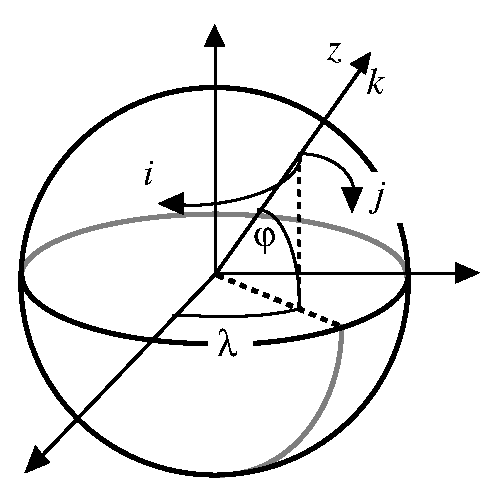
\includegraphics[width=0.60\textwidth]{./TexFiles/Figures/Fig_I_earth_referential.pdf}
\caption{	\label{Fig_referential} 
the geographical coordinate system $(\lambda,\varphi,z)$ and the curvilinear 
coordinate system (\textbf{i},\textbf{j},\textbf{k}). }
\end{center}   \end{figure}
%>>>>>>>>>>>>>>>>>>>>>>>>>>>>

Since the ocean depth is far smaller than the earth's radius, $a+z$, can be replaced by 
$a$ in (\ref{Eq_scale_factors}) (thin-shell approximation). The resulting horizontal scale 
factors $e_1$, $e_2$  are independent of $k$ while the vertical scale factor is a single 
function of $k$ as \textbf{k} is parallel to \textbf{z}. The scalar and vector operators that 
appear in the primitive equations (Eqs. \eqref{Eq_PE_dyn} to \eqref{Eq_PE_eos}) can 
be written in the tensorial form, invariant in any orthogonal horizontal curvilinear coordinate 
system transformation:
\begin{subequations} \label{Eq_PE_discrete_operators}
\begin{equation} \label{Eq_PE_grad}
\nabla q=\frac{1}{e_1 }\frac{\partial q}{\partial i}\;{\rm {\bf 
i}}+\frac{1}{e_2 }\frac{\partial q}{\partial j}\;{\rm {\bf j}}+\frac{1}{e_3 
}\frac{\partial q}{\partial k}\;{\rm {\bf k}}    \\
\end{equation}
\begin{equation} \label{Eq_PE_div}
\nabla \cdot {\rm {\bf A}} 
= \frac{1}{e_1 \; e_2} \left[ 
  \frac{\partial \left(e_2 \; a_1\right)}{\partial i }
+\frac{\partial \left(e_1 \; a_2\right)}{\partial j }    	\right]
+ \frac{1}{e_3} \left[ \frac{\partial a_3}{\partial k }   \right]
\end{equation}
\begin{equation} \label{Eq_PE_curl}
   \begin{split}
\nabla \times \vect{A} = 
    \left[ {\frac{1}{e_2 }\frac{\partial a_3}{\partial j}
            -\frac{1}{e_3 }\frac{\partial a_2 }{\partial k}} \right] \; \vect{i}
&+\left[ {\frac{1}{e_3 }\frac{\partial a_1 }{\partial k}
           -\frac{1}{e_1 }\frac{\partial a_3 }{\partial i}} \right] \; \vect{j} 		\\
&+\frac{1}{e_1 e_2 } \left[ {\frac{\partial \left( {e_2 a_2 } \right)}{\partial i}
                                       -\frac{\partial \left( {e_1 a_1 } \right)}{\partial j}} \right] \; \vect{k} 
   \end{split}
\end{equation}
\begin{equation} \label{Eq_PE_lap}
\Delta q = \nabla \cdot \left(  \nabla q \right)
\end{equation}
\begin{equation} \label{Eq_PE_lap_vector}
\Delta {\rm {\bf A}} =
  \nabla \left( \nabla \cdot {\rm {\bf A}} \right)
- \nabla \times \left(  \nabla \times {\rm {\bf A}} \right)
\end{equation}
\end{subequations}
where $q$ is a scalar quantity and ${\rm {\bf A}}=(a_1,a_2,a_3)$ a vector in the $(i,j,k)$ coordinate system.

% -------------------------------------------------------------------------------------------------------------
% Continuous Model Equations
% -------------------------------------------------------------------------------------------------------------
\subsection{Continuous Model Equations}
\label{PE_zco_Eq}

In order to express the Primitive Equations in tensorial formalism, it is necessary to compute 
the horizontal component of the non-linear and viscous terms of the equation using 
\eqref{Eq_PE_grad}) to \eqref{Eq_PE_lap_vector}. 
Let us set $\vect U=(u,v,w)={\vect{U}}_h +w\;\vect{k}$, the velocity in the $(i,j,k)$ coordinate 
system and define the relative vorticity $\zeta$ and the divergence of the horizontal velocity 
field $\chi$, by:
\begin{equation} \label{Eq_PE_curl_Uh}
\zeta =\frac{1}{e_1 e_2 }\left[ {\frac{\partial \left( {e_2 \,v} 
\right)}{\partial i}-\frac{\partial \left( {e_1 \,u} \right)}{\partial j}} 
\right]
\end{equation}
\begin{equation} \label{Eq_PE_div_Uh}
\chi =\frac{1}{e_1 e_2 }\left[ {\frac{\partial \left( {e_2 \,u} 
\right)}{\partial i}+\frac{\partial \left( {e_1 \,v} \right)}{\partial j}} 
\right]
\end{equation}

Using the fact that the horizontal scale factors $e_1$ and $e_2$ are independent of $k$ 
and that $e_3$  is a function of the single variable $k$, the nonlinear term of 
\eqref{Eq_PE_dyn} can be transformed as follows:
\begin{flalign*}
&\left[ {\left( {	\nabla \times {\rm {\bf U}}    } \right) \times {\rm {\bf U}}
+\frac{1}{2}	\nabla \left( {{\rm {\bf U}}^2} \right)}	 \right]_h 			&
\end{flalign*}
\begin{flalign*}
&\qquad=\left( {{\begin{array}{*{20}c}
 {\left[ 	{	 \frac{1}{e_3}	\frac{\partial u	}{\partial k}
			-\frac{1}{e_1}	\frac{\partial w	}{\partial i} } \right] w - \zeta \; v } 	 	\\
 		{\zeta \; u - \left[ {	 \frac{1}{e_2} \frac{\partial w}{\partial j}
							-\frac{1}{e_3} \frac{\partial v}{\partial k} } \right] \ w}	 \\
		 \end{array} }} \right)			
+\frac{1}{2}	\left( {{\begin{array}{*{20}c}
		 {	\frac{1}{e_1}	\frac{\partial \left( u^2+v^2+w^2 \right)}{\partial i}} 	\hfill	 \\
		 {	\frac{1}{e_2}	\frac{\partial \left( u^2+v^2+w^2 \right)}{\partial j}} 	\hfill	 \\
		 \end{array} }} \right)			&
\end{flalign*}
\begin{flalign*}
& \qquad =\left( {{	\begin{array}{*{20}c}
 {-\zeta \; v} \hfill \\
 { \zeta \; u} \hfill \\
			\end{array} }} \right)
+\frac{1}{2}\left( {{	\begin{array}{*{20}c}
 {\frac{1}{e_1 }\frac{\partial \left( {u^2+v^2} \right)}{\partial i}} \hfill 	\\
 {\frac{1}{e_2 }\frac{\partial \left( {u^2+v^2} \right)}{\partial j}} \hfill 	\\
						\end{array} }} \right)			
+\frac{1}{e_3 }\left( {{		\begin{array}{*{20}c}
 { w \; \frac{\partial u}{\partial k}} 	\\
 { w \; \frac{\partial v}{\partial k}} 	\\
							\end{array} }} \right)	
-\left( {{	\begin{array}{*{20}c}
 {\frac{w}{e_1}\frac{\partial w}{\partial i}
 -\frac{1}{2e_1}\frac{\partial w^2}{\partial i}} \hfill \\
 {\frac{w}{e_2}\frac{\partial w}{\partial j}
  -\frac{1}{2e_2}\frac{\partial w^2}{\partial j}} \hfill \\
			\end{array} }} \right) 			&
\end{flalign*}

The last term of the right hand side is obviously zero, and thus the nonlinear term of 
\eqref{Eq_PE_dyn} is written in the $(i,j,k)$ coordinate system:
\begin{equation} \label{Eq_PE_vector_form}
\left[ {\left( {	\nabla \times {\rm {\bf U}}    } \right) \times {\rm {\bf U}}
+\frac{1}{2}	\nabla \left( {{\rm {\bf U}}^2} \right)}	 \right]_h 
=\zeta 
\;{\rm {\bf k}}\times {\rm {\bf U}}_h +\frac{1}{2}\nabla _h \left( {{\rm 
{\bf U}}_h^2 } \right)+\frac{1}{e_3 }w\frac{\partial {\rm {\bf U}}_h 
}{\partial k}   	
\end{equation}

This is the so-called \textit{vector invariant form} of the momentum advection term. 
For some purposes, it can be advantageous to write this term in the so-called flux form, 
$i.e.$ to write it as the divergence of fluxes. For example, the first component of 
\eqref{Eq_PE_vector_form} (the $i$-component) is transformed as follows:
\begin{flalign*}
&{	\begin{array}{*{20}l}
\left[ {\left( {\nabla \times \vect{U}} \right)\times \vect{U}
          +\frac{1}{2}\nabla \left( {\vect{U}}^2 \right)} \right]_i   % \\
%\\
     = - \zeta \;v 
     + \frac{1}{2\;e_1 } \frac{\partial \left( {u^2+v^2} \right)}{\partial i}
     + \frac{1}{e_3}w \ \frac{\partial u}{\partial k} 			\\
\\
\qquad =\frac{1}{e_1 \; e_2} \left( 	-v\frac{\partial \left( {e_2 \,v} \right)}{\partial i}
							+v\frac{\partial \left( {e_1 \,u} \right)}{\partial j}	 \right)
+\frac{1}{e_1 e_2 }\left( 	+e_2 \; u\frac{\partial u}{\partial i}
 							+e_2 \; v\frac{\partial v}{\partial i}	  				 \right) 
+\frac{1}{e_3}       \left( 	w\;\frac{\partial u}{\partial k} 		\right)   \\
\end{array} } 			&
\end{flalign*}
\begin{flalign*}
&{	\begin{array}{*{20}l}
\qquad =\frac{1}{e_1 \; e_2} 	\left\{ 
 -\left(   	    v^2 	\frac{\partial e_2                                }{\partial i} 
 		+e_2 \,v		\frac{\partial v                                   }{\partial i}  	\right)
+\left( 				\frac{\partial \left( {e_1 \,u\,v} 	\right)}{\partial j}
		-e_1 \,u		\frac{\partial v                                   }{\partial j} 	\right) 	\right. 
\\  \left.	\qquad \qquad \quad
+\left( 				\frac{\partial \left( {e_2 u\,u}     \right)}{\partial i}
		-u			\frac{\partial \left( {e_2 u}         \right)}{\partial i} 	\right)
+e_2 v		 		\frac{\partial v                                    }{\partial i}
 						\right\} 
+\frac{1}{e_3} \left(
 					\frac{\partial \left( {w\,u} \right)         }{\partial k}
		 -u			\frac{\partial w 						   }{\partial k} 	\right) \\
\end{array} } 		&
\end{flalign*}
\begin{flalign*}
&{	\begin{array}{*{20}l}
\qquad =\frac{1}{e_1 \; e_2} 	\left( 
					\frac{\partial \left( {e_2 \,u\,u} \right)}{\partial i}
		+			\frac{\partial \left( {e_1 \,u\,v} \right)}{\partial j}	\right)
+\frac{1}{e_3 }		\frac{\partial \left( {w\,u		 } \right)}{\partial k}
\\  \qquad \qquad \quad
+\frac{1}{e_1 e_2 }		\left( 
 		-u	\left( 	\frac{\partial \left( {e_1 v	 } \right)}{\partial j}
	 				-v\,\frac{\partial e_1 }{\partial j}				 \right)
		-u			\frac{\partial \left( {e_2 u	 } \right)}{\partial i}
						\right)
 -\frac{1}{e_3 }	 	\frac{\partial w}{\partial k}	u
 +\frac{1}{e_1 e_2 }\left( 	-v^2\frac{\partial e_2	 }{\partial i}		 \right)	
\end{array} } 		&
\end{flalign*}
\begin{flalign*}
&{	\begin{array}{*{20}l}
\qquad = \nabla \cdot \left( {{\rm {\bf U}}\,u}	\right)
-   \left( \nabla \cdot {\rm {\bf U}} \right) \ u
+\frac{1}{e_1 e_2 }\left( 
		-v^2		\frac{\partial e_2 }{\partial i}
		+uv	\,		\frac{\partial e_1 }{\partial j} 	\right) \\
\end{array} } 		&
\end{flalign*}
as $\nabla \cdot {\rm {\bf U}}\;=0$ (incompressibility) it comes:
\begin{flalign*}
&{	\begin{array}{*{20}l}
\qquad = \nabla \cdot \left( 	{{\rm {\bf U}}\,u}		\right)
+	\frac{1}{e_1 e_2 }   \left( v \; \frac{\partial e_2}{\partial i}
						       -u \; \frac{\partial e_1}{\partial j} 	\right)  \left( -v \right)	
\end{array} } 		&
\end{flalign*}

The flux form of the momentum advection term is therefore given by:
\begin{multline} \label{Eq_PE_flux_form}
		\left[ 
  \left( 	{\nabla \times {\rm {\bf U}}} 	\right) \times {\rm {\bf U}}
+\frac{1}{2}	\nabla \left( 	{{\rm {\bf U}}^2} 	\right)
		\right]_h 
\\
= \nabla \cdot 	\left( {{\begin{array}{*{20}c}	{\rm {\bf U}} \, u 	\hfill \\
												{\rm {\bf U}} \, v	\hfill \\
						\end{array} }} 	
				\right)
+\frac{1}{e_1 e_2 }		\left( 
		 v\frac{\partial e_2}{\partial i}
		-u\frac{\partial e_1}{\partial j} 
						\right) {\rm {\bf k}} \times {\rm {\bf U}}_h
\end{multline}

The flux form has two terms, the first one is expressed as the divergence of momentum 
fluxes (hence the flux form name given to this formulation) and the second one is due to 
the curvilinear nature of the coordinate system used. The latter is called the \emph{metric} 
term and can be viewed as a modification of the Coriolis parameter: 
\begin{equation} \label{Eq_PE_cor+metric}
f \to f + \frac{1}{e_1\;e_2}  \left(  v \frac{\partial e_2}{\partial i}
					         -u \frac{\partial e_1}{\partial j}  \right)
\end{equation}

Note that in the case of geographical coordinate, $i.e.$ when $(i,j) \to (\lambda ,\varphi )$ 
and $(e_1 ,e_2) \to (a \,\cos \varphi ,a)$, we recover the commonly used modification of 
the Coriolis parameter $f \to f+(u/a) \tan \varphi$.


$\ $\newline    % force a new ligne

To sum up, the curvilinear $z$-coordinate equations solved by the ocean model can be 
written in the following tensorial formalism:

\vspace{+10pt}
$\bullet$ \textbf{Vector invariant form of the momentum equations} :

\begin{subequations} \label{Eq_PE_dyn_vect}
\begin{equation} \label{Eq_PE_dyn_vect_u} \begin{split}
\frac{\partial u}{\partial t} 
= +   \left( {\zeta +f} \right)\,v                                    
   -   \frac{1}{2\,e_1}           \frac{\partial}{\partial i} \left(  u^2+v^2   \right) 
   -   \frac{1}{e_3    }  w     \frac{\partial u}{\partial k}      &      \\
   -   \frac{1}{e_1    }            \frac{\partial}{\partial i} \left( \frac{p_s+p_h }{\rho _o}    \right)    
   &+   D_u^{\vect{U}}  +   F_u^{\vect{U}}      \\
\\
\frac{\partial v}{\partial t} =
       -   \left( {\zeta +f} \right)\,u   
       -   \frac{1}{2\,e_2 }        \frac{\partial }{\partial j}\left(  u^2+v^2  \right)   
       -   \frac{1}{e_3     }   w  \frac{\partial v}{\partial k}     &      \\
       -   \frac{1}{e_2     }        \frac{\partial }{\partial j}\left( \frac{p_s+p_h }{\rho _o}  \right)    
    &+  D_v^{\vect{U}}  +   F_v^{\vect{U}}
\end{split} \end{equation}
\end{subequations}


\vspace{+10pt}
$\bullet$ \textbf{flux form of the momentum equations} :
\begin{subequations} \label{Eq_PE_dyn_flux}
\begin{multline} \label{Eq_PE_dyn_flux_u}
\frac{\partial u}{\partial t}=
+   \left( { f + \frac{1}{e_1 \; e_2}
					\left( 	 v \frac{\partial e_2}{\partial i}
						-u \frac{\partial e_1}{\partial j} 	\right)} 	\right) \, v    \\
- \frac{1}{e_1 \; e_2} 	\left( 
					\frac{\partial \left( {e_2 \,u\,u} \right)}{\partial i}
		+			\frac{\partial \left( {e_1 \,v\,u} \right)}{\partial j}	\right)
                 - \frac{1}{e_3 }\frac{\partial \left( {         w\,u} \right)}{\partial k}    \\
-   \frac{1}{e_1 }\frac{\partial}{\partial i}\left( \frac{p_s+p_h }{\rho _o}   \right)
+   D_u^{\vect{U}} +   F_u^{\vect{U}}
\end{multline}
\begin{multline} \label{Eq_PE_dyn_flux_v}
\frac{\partial v}{\partial t}=
-   \left( { f + \frac{1}{e_1 \; e_2}
					\left( 	 v \frac{\partial e_2}{\partial i}
						-u \frac{\partial e_1}{\partial j} 	\right)} 	\right) \, u   \\
 \frac{1}{e_1 \; e_2} 	\left( 
					\frac{\partial \left( {e_2 \,u\,v} \right)}{\partial i}
		+			\frac{\partial \left( {e_1 \,v\,v} \right)}{\partial j}	\right)
                 - \frac{1}{e_3 } \frac{\partial \left( {        w\,v} \right)}{\partial k}    \\
-   \frac{1}{e_2 }\frac{\partial }{\partial j}\left( \frac{p_s+p_h }{\rho _o}    \right)
+  D_v^{\vect{U}} +  F_v^{\vect{U}} 
\end{multline}
\end{subequations}
where $\zeta$, the relative vorticity, is given by \eqref{Eq_PE_curl_Uh} and $p_s $, 
the surface pressure, is given by:
\begin{equation} \label{Eq_PE_spg}
p_s = \left\{ \begin{split} 
\rho \,g \,\eta &                                 \qquad  \qquad  \;   \qquad \text{ standard free surface} \\ 
\rho \,g \,\eta &+ \rho_o \,\mu \,\frac{\partial \eta }{\partial t}      \qquad \text{ filtered     free surface}    
\end{split} 
\right.
\end{equation}
with $\eta$ is solution of \eqref{Eq_PE_ssh}

The vertical velocity and the hydrostatic pressure are diagnosed from the following equations:
\begin{equation} \label{Eq_w_diag}
\frac{\partial w}{\partial k}=-\chi \;e_3 
\end{equation}
\begin{equation} \label{Eq_hp_diag}
\frac{\partial p_h }{\partial k}=-\rho \;g\;e_3 
\end{equation}
where the divergence of the horizontal velocity, $\chi$ is given by \eqref{Eq_PE_div_Uh}.

\vspace{+10pt}
$\bullet$ \textit{tracer equations} :
\begin{equation} \label{Eq_S}
\frac{\partial T}{\partial t} = 
-\frac{1}{e_1 e_2 }\left[ {	   \frac{\partial \left( {e_2 T\,u} \right)}{\partial i}
						+\frac{\partial \left( {e_1 T\,v} \right)}{\partial j}} \right]
-\frac{1}{e_3 }\frac{\partial \left( {T\,w} \right)}{\partial k} + D^T + F^T
\end{equation}
\begin{equation} \label{Eq_T}
\frac{\partial S}{\partial t} = 
-\frac{1}{e_1 e_2 }\left[ 	  {\frac{\partial \left( {e_2 S\,u} \right)}{\partial i}
						+\frac{\partial \left( {e_1 S\,v} \right)}{\partial j}} \right]
-\frac{1}{e_3 }\frac{\partial \left( {S\,w} \right)}{\partial k} + D^S + F^S
\end{equation}
\begin{equation} \label{Eq_rho}
\rho =\rho \left( {T,S,z(k)} \right)
\end{equation}

The expression of \textbf{D}$^{U}$, $D^{S}$ and $D^{T}$ depends on the subgrid scale 
parameterisation used. It will be defined in \S\ref{PE_zdf}. The nature and formulation of 
${\rm {\bf F}}^{\rm {\bf U}}$, $F^T$ and $F^S$, the surface forcing terms, are discussed 
in Chapter~\ref{SBC}.


\newpage 
$\ $\newline    % force a new ligne
% ================================================================
% Curvilinear generalised vertical coordinate System
% ================================================================
\section{Curvilinear generalised vertical coordinate System}
\label{PE_gco}

The ocean domain presents a huge diversity of situation in the vertical. First the ocean surface is a time dependent surface (moving surface). Second the ocean floor depends on the geographical position, varying from more than 6,000 meters in abyssal trenches to zero at the coast. Last but not least, the ocean stratification exerts a strong barrier to vertical motions and mixing. 
Therefore, in order to represent the ocean with respect to the first point a space and time dependent vertical coordinate that follows the variation of the sea surface height $e.g.$ an $z$*-coordinate; for the second point, a space variation to fit the change of bottom topography $e.g.$ a terrain-following or $\sigma$-coordinate; and for the third point, one will be tempted to use a space and time dependent coordinate that follows the isopycnal surfaces, $e.g.$ an isopycnic coordinate.

In order to satisfy two or more constrains one can even be tempted to mixed these coordinate systems, as in HYCOM (mixture of $z$-coordinate at the surface, isopycnic coordinate in the ocean interior and $\sigma$ at the ocean bottom) \citep{Chassignet_al_JPO03}  or OPA (mixture of $z$-coordinate in vicinity the surface and steep topography areas and $\sigma$-coordinate elsewhere) \citep{Madec_al_JPO96} among others.

In fact one is totally free to choose any space and time vertical coordinate by introducing an arbitrary vertical coordinate :
\begin{equation} \label{Eq_s}
s=s(i,j,k,t)
\end{equation}
with the restriction that the above equation gives a single-valued monotonic relationship between $s$ and $k$, when $i$, $j$ and $t$ are held fixed. \eqref{Eq_s} is a transformation from the $(i,j,k,t)$ coordinate system with independent variables into the $(i,j,s,t)$ generalised coordinate system with $s$ depending on the other three variables through \eqref{Eq_s}.
This so-called \textit{generalised vertical coordinate} \citep{Kasahara_MWR74} is in fact an Arbitrary Lagrangian--Eulerian (ALE) coordinate. Indeed, choosing an expression for $s$ is an arbitrary choice that determines which part of the vertical velocity (defined from a fixed referential) will cross the levels (Eulerian part) and which part will be used to move them (Lagrangian part).
The coordinate is also sometime referenced as an adaptive coordinate \citep{Hofmeister_al_OM09}, since the coordinate system is adapted in the course of the simulation. Its most often used implementation is via an ALE algorithm, in which a pure lagrangian step is followed by regridding and remapping steps, the later step implicitly embedding the vertical advection \citep{Hirt_al_JCP74, Chassignet_al_JPO03, White_al_JCP09}. Here we follow the \citep{Kasahara_MWR74} strategy : a regridding step (an update of the vertical coordinate) followed by an eulerian step with an explicit computation of vertical advection relative to the moving s-surfaces.

%\gmcomment{

%A key point here is that the $s$-coordinate depends on $(i,j)$ ==> horizontal pressure gradient...

the generalized vertical coordinates used in ocean modelling are not orthogonal, 
which contrasts with many other applications in mathematical physics. 
Hence, it is useful to keep in mind the following properties that may seem 
odd on initial encounter.

The horizontal velocity in ocean models measures motions in the horizontal plane, 
perpendicular to the local gravitational field. That is, horizontal velocity is mathematically 
the same regardless the vertical coordinate, be it geopotential, isopycnal, pressure, 
or terrain following. The key motivation for maintaining the same horizontal velocity 
component is that the hydrostatic and geostrophic balances are dominant in the large-scale ocean. 
Use of an alternative quasi-horizontal velocity, for example one oriented parallel 
to the generalized surface, would lead to unacceptable numerical errors. 
Correspondingly, the vertical direction is anti-parallel to the gravitational force in all 
of the coordinate systems. We do not choose the alternative of a quasi-vertical 
direction oriented normal to the surface of a constant generalized vertical coordinate. 

It is the method used to measure transport across the generalized vertical coordinate 
surfaces which differs between the vertical coordinate choices. That is, computation 
of the dia-surface velocity component represents the fundamental distinction between 
the various coordinates. In some models, such as geopotential, pressure, and 
terrain following, this transport is typically diagnosed from volume or mass conservation. 
In other models, such as isopycnal layered models, this transport is prescribed based 
on assumptions about the physical processes producing a flux across the layer interfaces. 


In this section we first establish the PE in the generalised vertical $s$-coordinate, 
then we discuss the particular cases available in \NEMO, namely $z$, $z$*, $s$, and $\tilde z$.  
%}

% -------------------------------------------------------------------------------------------------------------
% The s-coordinate Formulation
% -------------------------------------------------------------------------------------------------------------
\subsection{The \textit{s-}coordinate Formulation}

Starting from the set of equations established in \S\ref{PE_zco} for the special case $k=z$ 
and thus $e_3=1$, we introduce an arbitrary vertical coordinate $s=s(i,j,k,t)$, which includes 
$z$-, \textit{z*}- and $\sigma-$coordinates as special cases ($s=z$, $s=\textit{z*}$, and 
$s=\sigma=z/H$ or $=z/\left(H+\eta \right)$, resp.). A formal derivation of the transformed 
equations is given in Appendix~\ref{Apdx_A}. Let us define the vertical scale factor by 
$e_3=\partial_s z$  ($e_3$ is now a function of $(i,j,k,t)$ ), and the slopes in the 
(\textbf{i},\textbf{j}) directions between $s-$ and $z-$surfaces by :
\begin{equation} \label{Eq_PE_sco_slope}
\sigma _1 =\frac{1}{e_1 }\;\left. {\frac{\partial z}{\partial i}} \right|_s 
\quad \text{, and } \quad 
\sigma _2 =\frac{1}{e_2 }\;\left. {\frac{\partial z}{\partial j}} \right|_s
\end{equation}
We also introduce  $\omega $, a dia-surface velocity component, defined as the velocity 
relative to the moving $s$-surfaces and normal to them:
\begin{equation} \label{Eq_PE_sco_w}
\omega  = w - e_3 \, \frac{\partial s}{\partial t} - \sigma _1 \,u - \sigma _2 \,v    \\
\end{equation}

The equations solved by the ocean model \eqref{Eq_PE} in $s-$coordinate can be written as follows:

 \vspace{0.5cm}
* momentum equation:
\begin{multline} \label{Eq_PE_sco_u}
\frac{1}{e_3} \frac{\partial \left(  e_3\,u  \right) }{\partial t}=
	+   \left( {\zeta +f} \right)\,v                                    
	-   \frac{1}{2\,e_1} \frac{\partial}{\partial i} \left(  u^2+v^2   \right) 
	-   \frac{1}{e_3} \omega \frac{\partial u}{\partial k}       \\
	-   \frac{1}{e_1} \frac{\partial}{\partial i} \left( \frac{p_s + p_h}{\rho _o}    \right)    
	+  g\frac{\rho }{\rho _o}\sigma _1 
	+   D_u^{\vect{U}}  +   F_u^{\vect{U}} \quad
\end{multline}
\begin{multline} \label{Eq_PE_sco_v}
\frac{1}{e_3} \frac{\partial \left(  e_3\,v  \right) }{\partial t}=
	-   \left( {\zeta +f} \right)\,u   
	-   \frac{1}{2\,e_2 }\frac{\partial }{\partial j}\left(  u^2+v^2  \right)     	
	-   \frac{1}{e_3 } \omega \frac{\partial v}{\partial k}         \\
	-   \frac{1}{e_2 }\frac{\partial }{\partial j}\left( \frac{p_s+p_h }{\rho _o}  \right) 
	 +  g\frac{\rho }{\rho _o }\sigma _2   
	+  D_v^{\vect{U}}  +   F_v^{\vect{U}} \quad
\end{multline}
where the relative vorticity, \textit{$\zeta $}, the surface pressure gradient, and the hydrostatic 
pressure have the same expressions as in $z$-coordinates although they do not represent 
exactly the same quantities. $\omega$ is provided by the continuity equation 
(see Appendix~\ref{Apdx_A}):

\begin{equation} \label{Eq_PE_sco_continuity}
\frac{\partial e_3}{\partial t} + e_3 \; \chi + \frac{\partial \omega }{\partial s} = 0   
\qquad \text{with }\;\;  
\chi =\frac{1}{e_1 e_2 e_3 }\left[ {\frac{\partial \left( {e_2 e_3 \,u} 
\right)}{\partial i}+\frac{\partial \left( {e_1 e_3 \,v} \right)}{\partial 
j}} \right]
\end{equation}

 \vspace{0.5cm}
* tracer equations:
\begin{multline} \label{Eq_PE_sco_t}
\frac{1}{e_3} \frac{\partial \left(  e_3\,T  \right) }{\partial t}=
-\frac{1}{e_1 e_2 e_3 }\left[ {\frac{\partial \left( {e_2 e_3\,u\,T} \right)}{\partial i}
                                           +\frac{\partial \left( {e_1 e_3\,v\,T} \right)}{\partial j}} \right]   \\
-\frac{1}{e_3 }\frac{\partial \left( {T\,\omega } \right)}{\partial k}   + D^T + F^S   \qquad
\end{multline}

\begin{multline} \label{Eq_PE_sco_s}
\frac{1}{e_3} \frac{\partial \left(  e_3\,S  \right) }{\partial t}=
-\frac{1}{e_1 e_2 e_3 }\left[ {\frac{\partial \left( {e_2 e_3\,u\,S} \right)}{\partial i}
                                           +\frac{\partial \left( {e_1 e_3\,v\,S} \right)}{\partial j}} \right]    \\
-\frac{1}{e_3 }\frac{\partial \left( {S\,\omega } \right)}{\partial k}     + D^S + F^S   \qquad
\end{multline}

The equation of state has the same expression as in $z$-coordinate, and similar expressions 
are used for mixing and forcing terms.

\gmcomment{
\colorbox{yellow}{ to be updated $= = >$}
Add a few works on z and zps and s and underlies the differences between all of them
\colorbox{yellow}{ $< = =$ end update}  }



% -------------------------------------------------------------------------------------------------------------
% Curvilinear z*-coordinate System
% -------------------------------------------------------------------------------------------------------------
\subsection{Curvilinear \textit{z*}--coordinate System}
\label{PE_zco_star}

%>>>>>>>>>>>>>>>>>>>>>>>>>>>>
\begin{figure}[!b] 	 \begin{center}
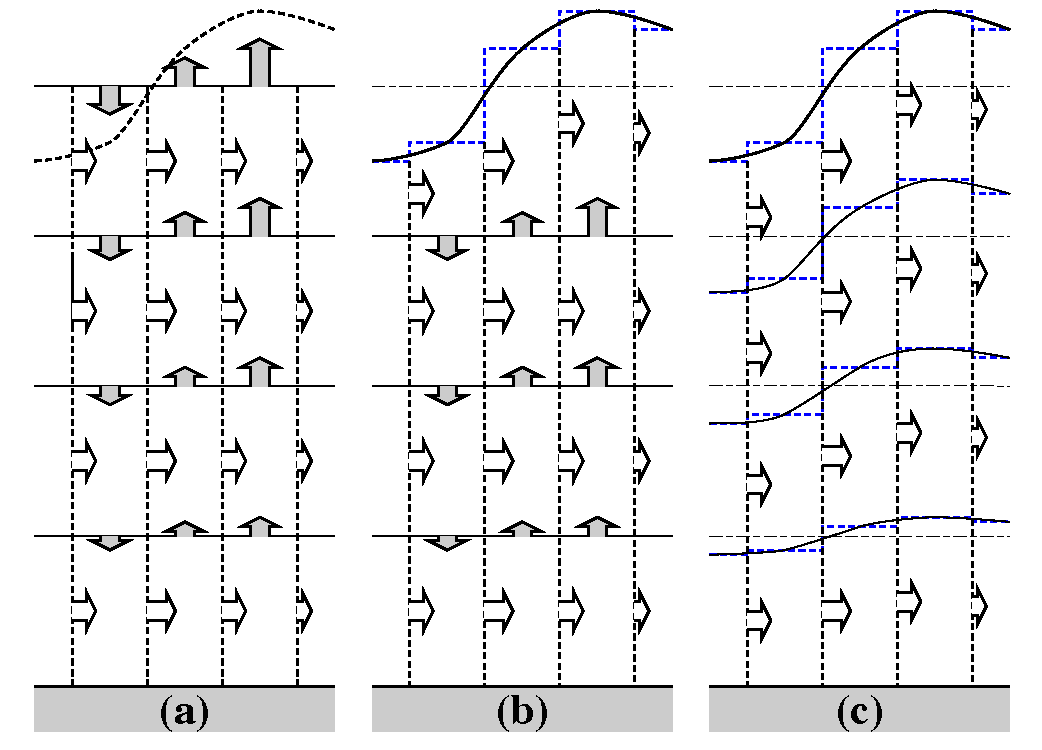
\includegraphics[width=1.0\textwidth]{./TexFiles/Figures/Fig_z_zstar.pdf}
\caption{	\label{Fig_z_zstar} 
(a) $z$-coordinate in linear free-surface case ; 
(b) $z-$coordinate in non-linear free surface case ; 
(c) re-scaled height coordinate (become popular as the \textit{z*-}coordinate 
\citep{Adcroft_Campin_OM04} ).}
\end{center}   \end{figure}
%>>>>>>>>>>>>>>>>>>>>>>>>>>>>


In that case, the free surface equation is nonlinear, and the variations of volume are fully 
taken into account. These coordinates systems is presented in a report \citep{Levier2007} 
available on the \NEMO web site. 

%\gmcomment{
The \textit{z*} coordinate approach is an unapproximated, non-linear free surface implementation 
which allows one to deal with large amplitude free-surface
variations relative to the vertical resolution \citep{Adcroft_Campin_OM04}. In
the  \textit{z*} formulation, the variation of the column thickness due to sea-surface
undulations is not concentrated in the surface level, as in the $z$-coordinate formulation,
but is equally distributed over the full water column. Thus vertical
levels naturally follow sea-surface variations, with a linear attenuation with
depth, as illustrated by figure fig.1c . Note that with a flat bottom, such as in
fig.1c, the bottom-following  $z$ coordinate and  \textit{z*} are equivalent.
The definition and modified oceanic equations for the rescaled vertical coordinate
 \textit{z*}, including the treatment of fresh-water flux at the surface, are
detailed in Adcroft and Campin (2004). The major points are summarized
here. The position ( \textit{z*}) and vertical discretization (\textit{z*}) are expressed as:
\begin{equation} \label{Eq_z-star}
H +  \textit{z*} = (H + z) / r \quad \text{and} \ \delta \textit{z*} = \delta z / r \quad \text{with} \ r = \frac{H+\eta} {H}
\end{equation} 
Since the vertical displacement of the free surface is incorporated in the vertical
coordinate  \textit{z*}, the upper and lower boundaries are at fixed  \textit{z*} position,  
$\textit{z*} = 0$ and  $\textit{z*} = -H$ respectively. Also the divergence of the flow field 
is no longer zero as shown by the continuity equation:
\begin{equation*} 
\frac{\partial r}{\partial t} = \nabla_{\textit{z*}} \cdot \left( r \; \rm{\bf U}_h \right)
		\left( r \; w\textit{*} \right) = 0 
\end{equation*} 
%}


% from MOM4p1 documentation

To overcome problems with vanishing surface and/or bottom cells, we consider the 
zstar coordinate 
\begin{equation} \label{PE_}
	z^\star = H \left( \frac{z-\eta}{H+\eta} \right)
\end{equation}

This coordinate is closely related to the "eta" coordinate used in many atmospheric 
models (see Black (1994) for a review of eta coordinate atmospheric models). It 
was originally used in ocean models by Stacey et al. (1995) for studies of tides 
next to shelves, and it has been recently promoted by Adcroft and Campin (2004) 
for global climate modelling.

The surfaces of constant $z^\star$ are quasi-horizontal. Indeed, the $z^\star$ coordinate reduces to $z$ when $\eta$ is zero. In general, when noting the large differences between 
undulations of the bottom topography versus undulations in the surface height, it 
is clear that surfaces constant $z^\star$ are very similar to the depth surfaces. These properties greatly reduce difficulties of computing the horizontal pressure gradient relative to terrain following sigma models discussed in \S\ref{PE_sco}. 
Additionally, since $z^\star$ when $\eta = 0$, no flow is spontaneously generated in an 
unforced ocean starting from rest, regardless the bottom topography. This behaviour is in contrast to the case with "s"-models, where pressure gradient errors in 
the presence of nontrivial topographic variations can generate nontrivial spontaneous flow from a resting state, depending on the sophistication of the pressure 
gradient solver. The quasi-horizontal nature of the coordinate surfaces also facilitates the implementation of neutral physics parameterizations in $z^\star$ models using 
the same techniques as in $z$-models (see Chapters 13-16 of \cite{Griffies_Bk04}) for a 
discussion of neutral physics in $z$-models, as well as Section \S\ref{LDF_slp} 
in this document for treatment in \NEMO). 

The range over which $z^\star$ varies is time independent $-H \leq z^\star \leq 0$. Hence, all 
cells remain nonvanishing, so long as the surface height maintains $\eta > ?H$. This 
is a minor constraint relative to that encountered on the surface height when using 
$s = z$ or $s = z - \eta$. 

Because $z^\star$ has a time independent range, all grid cells have static increments 
ds, and the sum of the ver tical increments yields the time independent ocean 
depth %�k ds = H. 
The $z^\star$ coordinate is therefore invisible to undulations of the 
free surface, since it moves along with the free surface. This proper ty means that 
no spurious ver tical transpor t is induced across surfaces of constant $z^\star$ by the 
motion of external gravity waves. Such spurious transpor t can be a problem in 
z-models, especially those with tidal forcing. Quite generally, the time independent 
range for the $z^\star$ coordinate is a very convenient proper ty that allows for a nearly 
arbitrary ver tical resolution even in the presence of large amplitude fluctuations of 
the surface height, again so long as $\eta > -H$. 

%end MOM doc %%%



\newpage 
% -------------------------------------------------------------------------------------------------------------
% Terrain following  coordinate System
% -------------------------------------------------------------------------------------------------------------
\subsection{Curvilinear Terrain-following \textit{s}--coordinate}
\label{PE_sco}

% -------------------------------------------------------------------------------------------------------------
% Introduction
% -------------------------------------------------------------------------------------------------------------
\subsubsection{Introduction}

Several important aspects of the ocean circulation are influenced by bottom topography. 
Of course, the most important is that bottom topography determines deep ocean sub-basins, 
barriers, sills and channels that strongly constrain the path of water masses, but more subtle 
effects exist. For example, the topographic $\beta$-effect is usually larger than the planetary 
one along continental slopes. Topographic Rossby waves can be excited and can interact 
with the mean current. In the $z-$coordinate system presented in the previous section 
(\S\ref{PE_zco}), $z-$surfaces are geopotential surfaces. The bottom topography is 
discretised by steps. This often leads to a misrepresentation of a gradually sloping bottom 
and to large localized depth gradients associated with large localized vertical velocities. 
The response to such a velocity field often leads to numerical dispersion effects. 
One solution to strongly reduce this error is to use a partial step representation of bottom 
topography instead of a full step one \cite{Pacanowski_Gnanadesikan_MWR98}. 
Another solution is to introduce a terrain-following coordinate system (hereafter $s-$coordinate) 

The $s$-coordinate avoids the discretisation error in the depth field since the layers of 
computation are gradually adjusted with depth to the ocean bottom. Relatively small 
topographic features as well as  gentle, large-scale slopes of the sea floor in the deep 
ocean, which would be ignored in typical $z$-model applications with the largest grid 
spacing at greatest depths, can easily be represented (with relatively low vertical resolution). 
A terrain-following model (hereafter $s-$model) also facilitates the modelling of the 
boundary layer flows over a large depth range, which in the framework of the $z$-model 
would require high vertical resolution over the whole depth range. Moreover, with a 
$s$-coordinate it is possible, at least in principle, to have the bottom and the sea surface 
as the only boundaries of the domain (nomore lateral boundary condition to specify). 
Nevertheless, a $s$-coordinate also has its drawbacks. Perfectly adapted to a 
homogeneous ocean, it has strong limitations as soon as stratification is introduced. 
The main two problems come from the truncation error in the horizontal pressure 
gradient and a possibly increased diapycnal diffusion. The horizontal pressure force 
in $s$-coordinate consists of two terms (see Appendix~\ref{Apdx_A}),

\begin{equation} \label{Eq_PE_p_sco}
\left. {\nabla p} \right|_z =\left. {\nabla p} \right|_s -\frac{\partial 
p}{\partial s}\left. {\nabla z} \right|_s 
\end{equation}

The second term in \eqref{Eq_PE_p_sco} depends on the tilt of the coordinate surface 
and introduces a truncation error that is not present in a $z$-model. In the special case 
of a $\sigma-$coordinate (i.e. a depth-normalised coordinate system $\sigma = z/H$), 
\citet{Haney1991} and \citet{Beckmann1993} have given estimates of the magnitude 
of this truncation error. It depends on topographic slope, stratification, horizontal and 
vertical resolution, the equation of state, and the finite difference scheme. This error 
limits the possible topographic slopes that a model can handle at a given horizontal 
and vertical resolution. This is a severe restriction for large-scale applications using 
realistic bottom topography. The large-scale slopes require high horizontal resolution, 
and the computational cost becomes prohibitive. This problem can be at least partially 
overcome by mixing $s$-coordinate and step-like representation of bottom topography \citep{Gerdes1993a,Gerdes1993b,Madec_al_JPO96}. However, the definition of the model 
domain vertical coordinate becomes then a non-trivial thing for a realistic bottom 
topography: a envelope topography is defined in $s$-coordinate on which a full or 
partial step bottom topography is then applied in order to adjust the model depth to 
the observed one (see \S\ref{DOM_zgr}.

For numerical reasons a minimum of diffusion is required along the coordinate surfaces 
of any finite difference model. It causes spurious diapycnal mixing when coordinate 
surfaces do not coincide with isoneutral surfaces. This is the case for a $z$-model as 
well as for a $s$-model. However, density varies more strongly on $s-$surfaces than 
on horizontal surfaces in regions of large topographic slopes, implying larger diapycnal 
diffusion in a $s$-model than in a $z$-model. Whereas such a diapycnal diffusion in a 
$z$-model tends to weaken horizontal density (pressure) gradients and thus the horizontal 
circulation, it usually reinforces these gradients in a $s$-model, creating spurious circulation. 
For example, imagine an isolated bump of topography in an ocean at rest with a horizontally 
uniform stratification. Spurious diffusion along $s$-surfaces will induce a bump of isoneutral 
surfaces over the topography, and thus will generate there a baroclinic eddy. In contrast, 
the ocean will stay at rest in a $z$-model. As for the truncation error, the problem can be reduced by introducing the terrain-following coordinate below the strongly stratified portion of the water column 
($i.e.$ the main thermocline) \citep{Madec_al_JPO96}. An alternate solution consists of rotating 
the lateral diffusive tensor to geopotential or to isoneutral surfaces (see \S\ref{PE_ldf}. 
Unfortunately, the slope of isoneutral surfaces relative to the $s$-surfaces can very large, 
strongly exceeding the stability limit of such a operator when it is discretized (see Chapter~\ref{LDF}). 

The $s-$coordinates introduced here \citep{Lott_al_OM90,Madec_al_JPO96} differ mainly in two 
aspects from similar models:  it allows  a representation of bottom topography with mixed 
full or partial step-like/terrain following topography ; It also offers a completely general 
transformation, $s=s(i,j,z)$ for the vertical coordinate.


\newpage 
% -------------------------------------------------------------------------------------------------------------
% Curvilinear z-tilde coordinate System
% -------------------------------------------------------------------------------------------------------------
\subsection{Curvilinear $\tilde{z}$--coordinate}
\label{PE_zco_tilde}

The $\tilde{z}$-coordinate has been developed by \citet{Leclair_Madec_OM10s}.
It is not available in the current version of \NEMO.

\newpage 
% ================================================================
% Subgrid Scale Physics
% ================================================================
\section{Subgrid Scale Physics}
\label{PE_zdf_ldf}

The primitive equations describe the behaviour of a geophysical fluid at 
space and time scales larger than a few kilometres in the horizontal, a few 
meters in the vertical and a few minutes. They are usually solved at larger 
scales: the specified grid spacing and time step of the numerical model. The 
effects of smaller scale motions (coming from the advective terms in the 
Navier-Stokes equations) must be represented entirely in terms of 
large-scale patterns to close the equations. These effects appear in the 
equations as the divergence of turbulent fluxes ($i.e.$ fluxes associated with 
the mean correlation of small scale perturbations). Assuming a turbulent 
closure hypothesis is equivalent to choose a formulation for these fluxes. 
It is usually called the subgrid scale physics. It must be emphasized that 
this is the weakest part of the primitive equations, but also one of the 
most important for long-term simulations as small scale processes \textit{in fine} 
balance the surface input of kinetic energy and heat.

The control exerted by gravity on the flow induces a strong anisotropy 
between the lateral and vertical motions. Therefore subgrid-scale physics  
\textbf{D}$^{\vect{U}}$, $D^{S}$ and $D^{T}$  in \eqref{Eq_PE_dyn}, 
\eqref{Eq_PE_tra_T} and \eqref{Eq_PE_tra_S} are divided into a lateral part  
\textbf{D}$^{l \vect{U}}$, $D^{lS}$ and $D^{lT}$ and a vertical part  
\textbf{D}$^{vU}$, $D^{vS}$ and $D^{vT}$. The formulation of these terms 
and their underlying physics are briefly discussed in the next two subsections.

% -------------------------------------------------------------------------------------------------------------
% Vertical Subgrid Scale Physics
% -------------------------------------------------------------------------------------------------------------
\subsection{Vertical Subgrid Scale Physics}
\label{PE_zdf}

The model resolution is always larger than the scale at which the major 
sources of vertical turbulence occur (shear instability, internal wave 
breaking...). Turbulent motions are thus never explicitly solved, even 
partially, but always parameterized. The vertical turbulent fluxes are 
assumed to depend linearly on the gradients of large-scale quantities (for 
example, the turbulent heat flux is given by $\overline{T'w'}=-A^{vT} \partial_z \overline T$, 
where $A^{vT}$ is an eddy coefficient). This formulation is 
analogous to that of molecular diffusion and dissipation. This is quite 
clearly a necessary compromise: considering only the molecular viscosity 
acting on large scale severely underestimates the role of turbulent 
diffusion and dissipation, while an accurate consideration of the details of 
turbulent motions is simply impractical. The resulting vertical momentum and 
tracer diffusive operators are of second order:
\begin{equation} \label{Eq_PE_zdf}
   \begin{split}
{\vect{D}}^{v \vect{U}} &=\frac{\partial }{\partial z}\left( {A^{vm}\frac{\partial {\vect{U}}_h }{\partial z}} \right) \ , \\         
D^{vT}                         &= \frac{\partial }{\partial z}\left( {A^{vT}\frac{\partial T}{\partial z}} \right) \ ,
\quad
D^{vS}=\frac{\partial }{\partial z}\left( {A^{vT}\frac{\partial S}{\partial z}} \right)
   \end{split}
\end{equation}
where $A^{vm}$ and $A^{vT}$ are the vertical eddy viscosity and diffusivity coefficients, 
respectively. At the sea surface and at the bottom, turbulent fluxes of momentum, heat 
and salt must be specified (see Chap.~\ref{SBC} and \ref{ZDF} and \S\ref{TRA_bbl}). 
All the vertical physics is embedded in the specification of the eddy coefficients. 
They can be assumed to be either constant, or function of the local fluid properties 
($e.g.$ Richardson number, Brunt-Vais\"{a}l\"{a} frequency...), or computed from a 
turbulent closure model. The choices available in \NEMO are discussed in \S\ref{ZDF}).

% -------------------------------------------------------------------------------------------------------------
% Lateral Diffusive and Viscous Operators Formulation
% -------------------------------------------------------------------------------------------------------------
\subsection{Formulation of the Lateral Diffusive and Viscous Operators}
\label{PE_ldf}

Lateral turbulence can be roughly divided into a mesoscale turbulence 
associated with eddies (which can be solved explicitly if the resolution is 
sufficient since their underlying physics are included in the primitive 
equations), and a sub mesoscale turbulence which is never explicitly solved 
even partially, but always parameterized. The formulation of lateral eddy 
fluxes depends on whether the mesoscale is below or above the grid-spacing 
($i.e.$ the model is eddy-resolving or not).

In non-eddy-resolving configurations, the closure is similar to that used 
for the vertical physics. The lateral turbulent fluxes are assumed to depend 
linearly on the lateral gradients of large-scale quantities. The resulting 
lateral diffusive and dissipative operators are of second order. 
Observations show that lateral mixing induced by mesoscale turbulence tends 
to be along isopycnal surfaces (or more precisely neutral surfaces \cite{McDougall1987}) 
rather than across them. 
As the slope of neutral surfaces is small in the ocean, a common 
approximation is to assume that the `lateral' direction is the horizontal, 
$i.e.$ the lateral mixing is performed along geopotential surfaces. This leads 
to a geopotential second order operator for lateral subgrid scale physics. 
This assumption can be relaxed: the eddy-induced turbulent fluxes can be 
better approached by assuming that they depend linearly on the gradients of 
large-scale quantities computed along neutral surfaces. In such a case, 
the diffusive operator is an isoneutral second order operator and it has 
components in the three space directions. However, both horizontal and 
isoneutral operators have no effect on mean ($i.e.$ large scale) potential 
energy whereas potential energy is a main source of turbulence (through 
baroclinic instabilities). \citet{Gent1990} have proposed a 
parameterisation of mesoscale eddy-induced turbulence which associates an 
eddy-induced velocity to the isoneutral diffusion. Its mean effect is to 
reduce the mean potential energy of the ocean. This leads to a formulation 
of lateral subgrid-scale physics made up of an isoneutral second order 
operator and an eddy induced advective part. In all these lateral diffusive 
formulations, the specification of the lateral eddy coefficients remains the 
problematic point as there is no really satisfactory formulation of these 
coefficients as a function of large-scale features.

In eddy-resolving configurations, a second order operator can be used, but 
usually the more scale selective biharmonic operator is preferred as the 
grid-spacing is usually not small enough compared to the scale of the 
eddies. The role devoted to the subgrid-scale physics is to dissipate the 
energy that cascades toward the grid scale and thus to ensure the stability of 
the model while not interfering with the resolved mesoscale activity. Another approach 
is becoming more and more popular: instead of specifying explicitly a sub-grid scale 
term in the momentum and tracer time evolution equations, one uses a advective 
scheme which is diffusive enough to maintain the model stability. It must be emphasised
that then, all the sub-grid scale physics is included in the formulation of the
advection scheme. 

All these parameterisations of subgrid scale physics have advantages and 
drawbacks. There are not all available in \NEMO. In the $z$-coordinate 
formulation, five options are offered for active tracers (temperature and 
salinity): second order geopotential operator, second order isoneutral 
operator, \citet{Gent1990} parameterisation, fourth order 
geopotential operator, and various slightly diffusive advection schemes. 
The same options are available for momentum, except 
\citet{Gent1990} parameterisation which only involves tracers. In the
$s$-coordinate formulation, additional options are offered for tracers: second 
order operator acting along $s-$surfaces, and for momentum: fourth order 
operator acting along $s-$surfaces (see \S\ref{LDF}).

\subsubsection{Lateral second order tracer diffusive operator}

The lateral second order tracer diffusive operator is defined by (see Appendix~\ref{Apdx_B}):
\begin{equation} \label{Eq_PE_iso_tensor}
D^{lT}=\nabla {\rm {\bf .}}\left( {A^{lT}\;\Re \;\nabla T} \right) \qquad 
\mbox{with}\quad \;\;\Re =\left( {{\begin{array}{*{20}c}
 1 \hfill & 0 \hfill & {-r_1 } \hfill \\
 0 \hfill & 1 \hfill & {-r_2 } \hfill \\
 {-r_1 } \hfill & {-r_2 } \hfill & {r_1 ^2+r_2 ^2} \hfill \\
\end{array} }} \right)
\end{equation}
where $r_1 \;\mbox{and}\;r_2 $ are the slopes between the surface along 
which the diffusive operator acts and the model level ($e. g.$ $z$- or 
$s$-surfaces). Note that the formulation \eqref{Eq_PE_iso_tensor} is exact for the 
rotation between geopotential and $s$-surfaces, while it is only an approximation 
for the rotation between isoneutral and $z$- or $s$-surfaces. Indeed, in the latter 
case, two assumptions are made to simplify  \eqref{Eq_PE_iso_tensor} \citep{Cox1987}. 
First, the horizontal contribution of the dianeutral mixing is neglected since the ratio 
between iso and dia-neutral diffusive coefficients is known to be several orders of 
magnitude smaller than unity. Second, the two isoneutral directions of diffusion are 
assumed to be independent since the slopes are generally less than $10^{-2}$ in the 
ocean (see Appendix~\ref{Apdx_B}).

For \textit{geopotential} diffusion, $r_1$ and $r_2 $ are the slopes between the 
geopotential and computational surfaces: in $z$-coordinates they are zero 
($r_1 = r_2 = 0$) while in $s$-coordinate (including $\textit{z*}$ case) they are 
equal to $\sigma _1$ and $\sigma _2$, respectively (see \eqref{Eq_PE_sco_slope} ).

For \textit{isoneutral} diffusion $r_1$ and $r_2$ are the slopes between the isoneutral 
and computational surfaces. Therefore, they are different quantities,
but have similar expressions in $z$- and $s$-coordinates. In $z$-coordinates:
\begin{equation} \label{Eq_PE_iso_slopes}
r_1 =\frac{e_3 }{e_1 }	\left( {\frac{\partial \rho }{\partial i}} \right)
						\left( {\frac{\partial \rho }{\partial k}} \right)^{-1} \ , \quad
r_1 =\frac{e_3 }{e_1 }	\left( {\frac{\partial \rho }{\partial i}} \right)
						\left( {\frac{\partial \rho }{\partial k}} \right)^{-1},
\end{equation}
while in $s$-coordinates $\partial/\partial k$ is replaced by
$\partial/\partial s$.

\subsubsection{Eddy induced velocity}
 When the \textit{eddy induced velocity} parametrisation (eiv) \citep{Gent1990} is used, 
an additional tracer advection is introduced in combination with the isoneutral diffusion of tracers:
\begin{equation} \label{Eq_PE_iso+eiv}
D^{lT}=\nabla \cdot \left( {A^{lT}\;\Re \;\nabla T} \right)
           +\nabla \cdot \left( {{\vect{U}}^\ast \,T} \right)
\end{equation}
where ${\vect{U}}^\ast =\left( {u^\ast ,v^\ast ,w^\ast } \right)$ is a non-divergent, 
eddy-induced transport velocity. This velocity field is defined by:
\begin{equation} \label{Eq_PE_eiv}
   \begin{split}
 u^\ast  &= +\frac{1}{e_3       }\frac{\partial }{\partial k}\left[ {A^{eiv}\;\tilde{r}_1 } \right] \\ 
 v^\ast  &= +\frac{1}{e_3       }\frac{\partial }{\partial k}\left[ {A^{eiv}\;\tilde{r}_2 } \right] \\ 
 w^\ast &=  -\frac{1}{e_1 e_2 }\left[ 
                      \frac{\partial }{\partial i}\left( {A^{eiv}\;e_2\,\tilde{r}_1 } \right)
                    +\frac{\partial }{\partial j}\left( {A^{eiv}\;e_1\,\tilde{r}_2 } \right)      \right]
   \end{split}
\end{equation}
where $A^{eiv}$ is the eddy induced velocity coefficient (or equivalently the isoneutral 
thickness diffusivity coefficient), and $\tilde{r}_1$ and $\tilde{r}_2$ are the slopes 
between isoneutral and \emph{geopotential} surfaces. Their values are
thus independent of the vertical coordinate, but their expression depends on the coordinate: 
\begin{align} \label{Eq_PE_slopes_eiv}
\tilde{r}_n = \begin{cases}
   r_n                  &      \text{in $z$-coordinate}    \\
   r_n + \sigma_n &      \text{in \textit{z*} and $s$-coordinates}  
                   \end{cases}
\quad \text{where } n=1,2
\end{align}

The normal component of the eddy induced velocity is zero at all the boundaries. 
This can be achieved in a model by tapering either the eddy coefficient or the slopes 
to zero in the vicinity of the boundaries. The latter strategy is used in \NEMO (cf. Chap.~\ref{LDF}).

\subsubsection{Lateral fourth order tracer diffusive operator}

The lateral fourth order tracer diffusive operator is defined by:
\begin{equation} \label{Eq_PE_bilapT}
D^{lT}=\Delta \left( {A^{lT}\;\Delta T} \right) 
\qquad \text{where} \  D^{lT}=\Delta \left( {A^{lT}\;\Delta T} \right)
 \end{equation}

It is the second order operator given by \eqref{Eq_PE_iso_tensor} applied twice with 
the eddy diffusion coefficient correctly placed. 


\subsubsection{Lateral second order momentum diffusive operator}

The second order momentum diffusive operator along $z$- or $s$-surfaces is found by 
applying \eqref{Eq_PE_lap_vector} to the horizontal velocity vector (see Appendix~\ref{Apdx_B}):
\begin{equation} \label{Eq_PE_lapU}
\begin{split}
{\rm {\bf D}}^{l{\rm {\bf U}}} 
&= \quad \  \nabla _h \left( {A^{lm}\chi } \right)
   \ - \ \nabla _h \times \left( {A^{lm}\,\zeta \;{\rm {\bf k}}} \right)     \\
&=   \left(      \begin{aligned}
             \frac{1}{e_1      } \frac{\partial \left( A^{lm} \chi          \right)}{\partial i} 
         &-\frac{1}{e_2 e_3}\frac{\partial \left( {A^{lm} \;e_3 \zeta} \right)}{\partial j}  \\
             \frac{1}{e_2      }\frac{\partial \left( {A^{lm} \chi         } \right)}{\partial j}   
         &+\frac{1}{e_1 e_3}\frac{\partial \left( {A^{lm} \;e_3 \zeta} \right)}{\partial i}
        \end{aligned}    \right)
\end{split}
\end{equation}

Such a formulation ensures a complete separation between the vorticity and 
horizontal divergence fields (see Appendix~\ref{Apdx_C}). Unfortunately, it is not 
available for geopotential diffusion in $s-$coordinates and for isoneutral 
diffusion in both $z$- and $s$-coordinates ($i.e.$ when a rotation is required). 
In these two cases, the $u$ and $v-$fields are considered as independent scalar 
fields, so that the diffusive operator is given by:
\begin{equation} \label{Eq_PE_lapU_iso}
\begin{split}
 D_u^{l{\rm {\bf U}}} &= \nabla .\left( {\Re \;\nabla u} \right) \\ 
 D_v^{l{\rm {\bf U}}} &= \nabla .\left( {\Re \;\nabla v} \right)
 \end{split}
 \end{equation}
where $\Re$ is given by  \eqref{Eq_PE_iso_tensor}. It is the same expression as 
those used for diffusive operator on tracers. It must be emphasised that such a 
formulation is only exact in a Cartesian coordinate system, $i.e.$ on a $f-$ or 
$\beta-$plane, not on the sphere. It is also a very good approximation in vicinity 
of the Equator in a geographical coordinate system \citep{Lengaigne_al_JGR03}.

\subsubsection{lateral fourth order momentum diffusive operator}

As for tracers, the fourth order momentum diffusive operator along $z$ or $s$-surfaces 
is a re-entering second order operator \eqref{Eq_PE_lapU} or \eqref{Eq_PE_lapU} 
with the eddy viscosity coefficient correctly placed:

geopotential diffusion in $z$-coordinate:
\begin{equation} \label{Eq_PE_bilapU}
\begin{split}
{\rm {\bf D}}^{l{\rm {\bf U}}} &=\nabla _h \left\{ {\;\nabla _h {\rm {\bf 
.}}\left[ {A^{lm}\,\nabla _h \left( \chi \right)} \right]\;} 
\right\}\;   \\
&+\nabla _h \times \left\{ {\;{\rm {\bf k}}\cdot \nabla \times 
\left[ {A^{lm}\,\nabla _h \times \left( {\zeta \;{\rm {\bf k}}} \right)} 
\right]\;} \right\}
\end{split}
\end{equation}

\gmcomment{  change the position of the coefficient, both here and in the code}

geopotential diffusion in $s$-coordinate:
\begin{equation} \label{Eq_bilapU_iso}
   \left\{   \begin{aligned}
         D_u^{l{\rm {\bf U}}} =\Delta \left( {A^{lm}\;\Delta u} \right) \\ 
         D_v^{l{\rm {\bf U}}} =\Delta \left( {A^{lm}\;\Delta v} \right)
   \end{aligned}    \right.
   \quad \text{where} \quad 
   \Delta \left( \bullet \right) = \nabla \cdot \left( \Re \nabla(\bullet) \right) 
\end{equation}

